%%%% Proceedings format for most of ACM conferences (with the exceptions listed below) and all ICPS volumes.
\documentclass[sigconf]{acmart}
\usepackage{graphicx}
\graphicspath{{imgs/}}
\usepackage[english,ngerman,brazilian]{babel}
\settopmatter{printacmref=false}
\setcopyright{none}
\renewcommand\footnotetextcopyrightpermission[1]{}
\pagestyle{plain}

\def\BibTeX{{\rm B\kern-.05em{\sc i\kern-.025em b}\kern-.08emT\kern-.1667em\lower.7ex\hbox{E}\kern-.125emX}}

% end of the preamble, start of the body of the document source.
\begin{document}

%
% The "title" command has an optional parameter, allowing the author to define a "short title" to be used in page headers.
\title[Fronteiras da Transferência de Aprendizado: uma revisão sistemática com enfoque meta-analítico]{Fronteiras da Transferência de Aprendizado: \\
uma revisão sistemática com enfoque meta-analítico}
%

\author{Fred Guth}
% \authornote{Both authors contributed equally to this research.}
\email{fredguth@fredguth.com}
\affiliation{%
  \institution{Departamento de Ciência de Computação, Universidade de Brasília}
  \postcode{70.910-900}
  \city{Brasília}
  \state{DF}
  \country{Brazil}
}

\renewcommand{\shortauthors}{Guth, F.}

%
% The abstract is a short summary of the work to be presented in the article.
\begin{abstract}
  Humanos e animais conseguem aprender com poucas amostras \cite{goodfellow} e apresentam extraordinária capacidade de generalização que os algoritmos de aprendizagem de máquina ainda estão longe de alcançar. Os modelos mais bem sucedidos da atualidade exigem uma enormidade de dados bem rotulados que são caros e difíceis de obter, tornando-se hoje um dos maiores empecilhos para aplicações práticas. Esse cenário prova o grande potencial da área de Transferência de Aprendizado, que tem por objetivo aproveitar o conhecimento obtido em uma atividade para aprender mais eficientemente outras, que guardem alguma relação com a primeira. O presente estudo visa apresentar uma revisão sistemática da literatura e identificar, com embasamento quantitativo, as principais contribuições para a área. Além disso, usamos o acoplamento bibliográfico para identificar trabalhos na fronteira do conhecimento e fizemos uma análise textual, em resumos e palavras-chave, comparando estes com os "clássicos" da área de forma a mapear para que direção a pesquisa avança.  
\end{abstract}

%   O objetivo deste estudo é mostrar uma revisão sistemática da literatura com as principais contribuições em transferência de aprendizagem. Uma pesquisa exploratória foi realizada, de abordagem quantitativa, por meio da Teoria do Enfoque Meta Analítico Consolidado
% Esta pesquisa quer responder: quais são as fronteiras do conhecimento em transferência de aprendizagem?  É possível embasar essa avaliação em dados bibliométricos?
%   Os melhores casos de sucesso foram desenvolvidos exclusiva
%
% The code below is generated by the tool at http://dl.acm.org/ccs.cfm.
% Please copy and paste the code instead of the example below.
%

\begin{CCSXML}
<ccs2012>
 <concept>
 <concept_id>10010147.10010257.10010258.10010262.10010277</concept_id>
 <concept_desc>Computing methodologies~Transfer learning</concept_desc>
 <concept_significance>500</concept_significance>
 </concept>
</ccs2012>
\end{CCSXML}
\ccsdesc[500]{Computing methodologies~Transfer learning}

\keywords{transferência de aprendizado, revisão sistemática, enfoque meta-analítico}

%
% A "teaser" image appears between the author and affiliation information and the body 
% of the document, and typically spans the page. 
% \begin{teaserfigure}
%   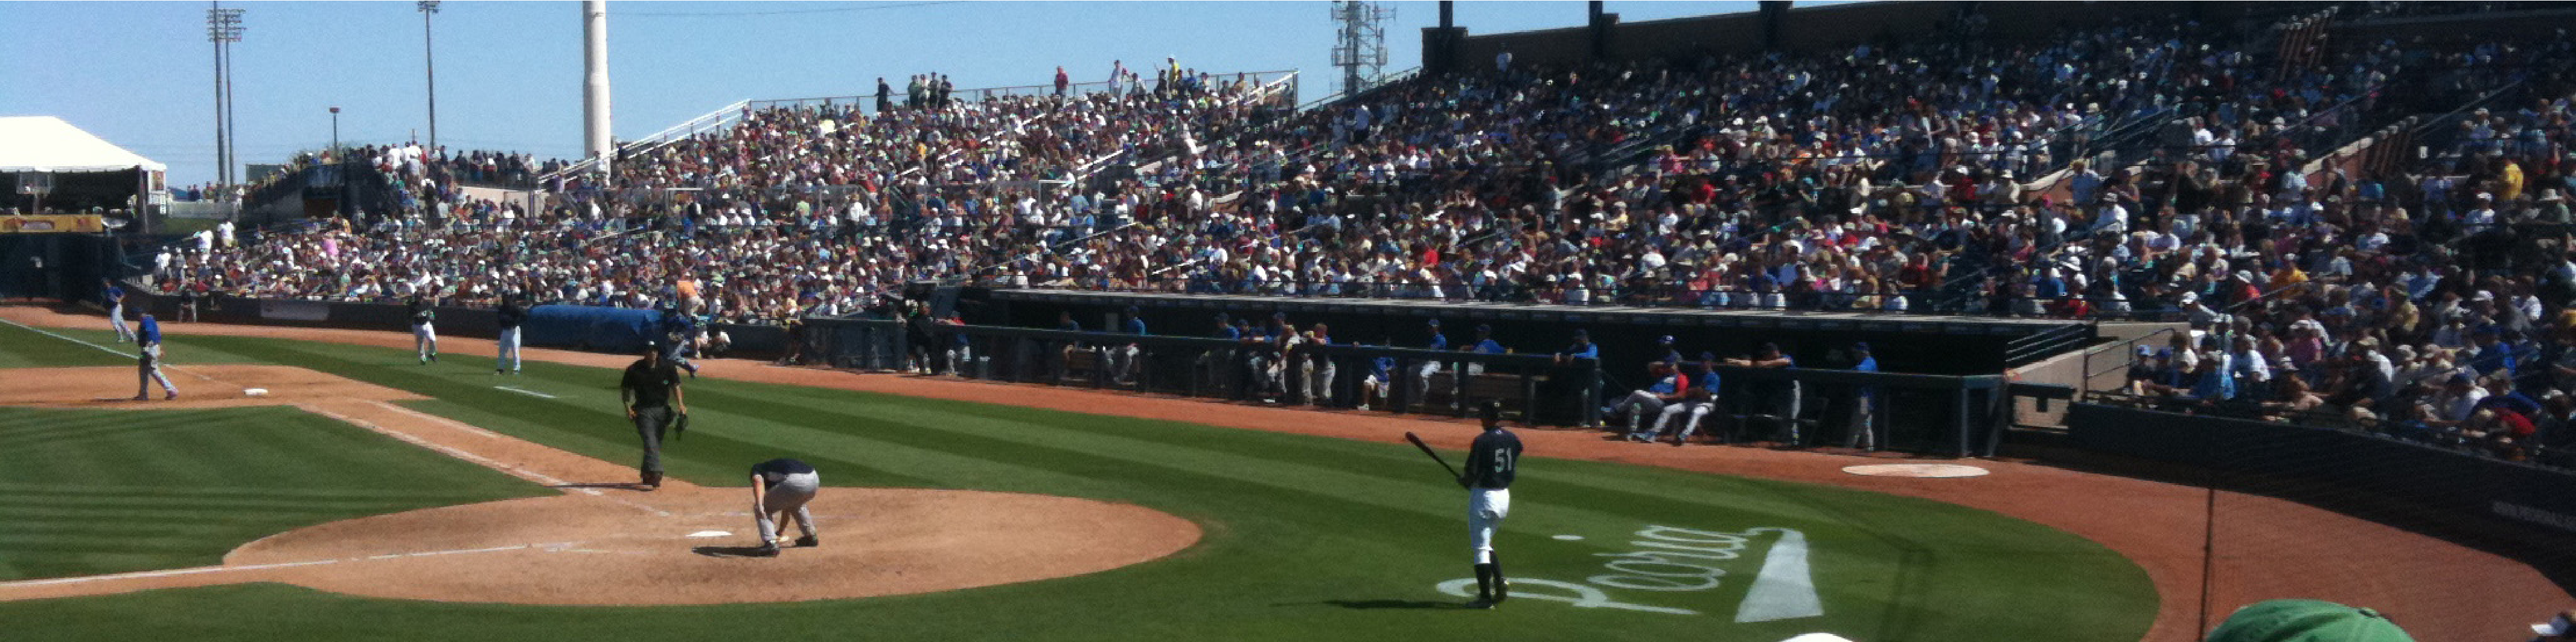
\includegraphics[width=\textwidth]{sampleteaser}
%   \caption{Seattle Mariners at Spring Training, 2010.}
%   \Description{Enjoying the baseball game from the third-base seats. Ichiro Suzuki preparing to bat.}
%   \label{fig:teaser}
% \end{teaserfigure}

\maketitle


\section{Introdução} 
  \subsection{Contribuições}
  \subsection{Visão Geral e Organização do Artigo}
  \subsection{Trabalhos Relacionados}
\section{Método de Revisão Sistemática}
  \subsection{O Enfoque Meta Analítico}
  \subsection{Análise de Co-citações}
  \subsection{Análise de Acoplamento Bibliográfico}
  \subsection{Análise Textual}
  \subsection{Sumarização}
\section{Revisão da Literatura}
  \subsection{Transferência de Aprendizagem}
  \subsection{Um breve histórico}
  \subsection{Os Clássicos}
  \subsection{A Fronteira}
\section{Problemas em Aberto}
\section{Conclusão}
\bibliographystyle{ACM-Reference-Format}
\bibliography{references}
\end{document}
